\documentclass[11pt,a4paper]{ctexart}
\usepackage[margin=2cm]{geometry}
\usepackage{amsmath,amssymb,bm}
\usepackage{booktabs,graphicx,xcolor,hyperref}
\hypersetup{colorlinks=true,linkcolor=blue,urlcolor=blue}
\setlength{\parindent}{2em}
\setlength{\parskip}{0.25em}
\title{IMU--UWB InEKF：结构化低开销实现与闭式惯性传播}
\author{基于改进版右不变协方差/门限实现}
\date{2026年7月23日}

\begin{document}
\maketitle

\section{范围与原论文对照}

原论文保留 15 维右不变误差状态
\begin{equation}
 \delta x=[\delta\theta,\delta v,\delta p,\delta b_g,\delta b_a],
\end{equation}
并在式 (40) 使用
\begin{equation}
 \Phi=\exp(A\Delta t),\qquad
 P^-=\Phi P^+\Phi^{\mathsf T}+LQL^{\mathsf T}\Delta t.
\end{equation}
本版建立在已经修复的偏置顺序、事件时间、右不变协方差初始化、同坐标 NIS
门限和全圆 yaw 先验之上，不撤销这些改进，也不切换滤波器主题。

\section{精确有限阶状态转移}

当前冻结区间内的传播矩阵可写为
\begin{equation}
 A=\begin{bmatrix}A_0&B\\0&0\end{bmatrix},\qquad
 A_0=\begin{bmatrix}
 0&0&0\\g^\times&0&0\\0&I&0
 \end{bmatrix}.
\end{equation}
虽然 $B$ 随当前姿态、速度和位置改变，但每个区间内 $B$ 为常量，而且
$A_0^3=0$，故
\begin{equation}
 A^4=\begin{bmatrix}A_0^4&A_0^3B\\0&0\end{bmatrix}=0.
\end{equation}
因此报告中这一建议在当前模型上成立，通用矩阵指数可被严格等价地替换为
\begin{equation}
 \boxed{\Phi=I+A\Delta t+\frac12A^2\Delta t^2+
 \frac16A^3\Delta t^3.}
 \label{eq:phi}
\end{equation}
单元测试将式~\eqref{eq:phi} 与 SciPy \texttt{expm} 比较到约
$10^{-15}$ 量级。

\section{稀疏噪声与标量秩一更新}

公开参数在当前生产路径中保留“每 IMU 样本方差”的既有语义。令
\begin{equation}
 D=\operatorname{diag}(q_1,\ldots,q_{15})\Delta t^2,\qquad
 M=\Phi\operatorname{Ad}_{\hat X,\hat b},
\end{equation}
其中位置噪声三列严格为零。过程噪声直接按列缩放：
\begin{equation}
 Q_d=MDM^{\mathsf T}
 =\left(M\operatorname{diag}(q_i\Delta t^2)\right)M^{\mathsf T},
\end{equation}
避免构造零块和四次连续稠密乘法；该式与旧稠密公式逐元素一致。

对一维 TDoA 量测，令
\begin{equation}
 u=P^-H^{\mathsf T},\qquad S=Hu+R.
\end{equation}
则采用
\begin{align}
 K&=u/S,\\
 \delta x&=u\,r/S,\\
 \boxed{P^+=P^--uu^{\mathsf T}/S.}
\end{align}
它与原论文式 (24) 的 Joseph 形式在精确算术下等价；实现仍进行对称化并检查
$S>0$。单元测试验证两种更新的状态和协方差一致。

\section{不构造增广伴随的现有 Jacobian}

本版保留已经通过大 yaw 数据验证的
$H_r=H_l\operatorname{Ad}_{\hat X^{-1}}$ 观测路径，而不是启用研究模式中尚未成熟的
完整杆臂 Jacobian。若 $h_p$ 是 $H_l$ 的位置行，直接写成
\begin{equation}
 \boxed{
 H_r=
 \begin{bmatrix}
 -h_pR^{\mathsf T}p^\times&0&h_pR^{\mathsf T}&0&0
 \end{bmatrix}.}
\end{equation}
该式与原来的 $15\times15$ 增广伴随乘法通过逐元素回归测试。

\section{闭式 IMU 积分}

原论文式 (39) 在一个采样区间内固定姿态作用于比力。对常角速度和常体坐标比力，
令 $\phi=(\omega-b_g)\Delta t$，本版使用
\begin{align}
 R_{k+1}&=R_k\operatorname{Exp}(\phi),\\
 v_{k+1}&=v_k+g\Delta t+
 R_k\Gamma_1(\phi)(a-b_a)\Delta t,\\
 p_{k+1}&=p_k+v_k\Delta t+\tfrac12g\Delta t^2+
 R_k\Gamma_2(\phi)(a-b_a)\Delta t^2,
\end{align}
其中
\begin{align}
 \Gamma_1(\phi)
 &=I+\frac{1-\cos\theta}{\theta^2}\phi^\times
 +\frac{\theta-\sin\theta}{\theta^3}(\phi^\times)^2,\\
 \Gamma_2(\phi)
 &=\frac12I+\frac{\theta-\sin\theta}{\theta^3}\phi^\times
 +\frac{\theta^2+2\cos\theta-2}{2\theta^4}(\phi^\times)^2.
\end{align}
$\operatorname{Exp}$、$\Gamma_1$、$\Gamma_2$ 共用一次叉乘矩阵、一次平方以及同一组
$\sin/\cos$；小角度使用连续级数。$\Gamma_2$ 已对高分辨率数值积分验证。

\section{被审计但未机械采用的建议}

\begin{itemize}
 \item 分块维护 $P$：在 Python/NumPy 中大量 $3\times3$ 切片和解释器循环未必比
 固定的 $15\times15$ BLAS 更快，且增加索引错误风险；本轮只消除了可证明的零块
 构造与乘法。嵌入式 C/C++ 版本仍适合继续展开。
 \item 连续 PSD 的有限阶 $Q_d$：当前生产参数是每样本方差，直接改成连续谱密度会
 改变调谐含义；研究模式已有 Van Loan 对照，因此本轮不偷换噪声模型。
 \item 自适应/Huber UWB：坐标不一致导致的大 yaw 门限闭锁已经修复；缺少冻结的
 分锚点对标定和独立验证前，不用在线自适应掩盖模型误差。
 \item 协方差降频、冻结偏置和 15/9 维切换：均为近似且可能损害温漂与大机动性能，
 不作为默认路径。
\end{itemize}

\section{数据结果}

\begin{table}[htbp]
\centering
\caption{当前改进基线与结构化版本的交错顺序配对结果}
\begin{tabular}{lrrrrr}
\toprule
数据 & 耗时前/s & 耗时后/s & 加速 & 位置前/后 m & yaw前/后 rad\\
\midrule
const1 自动 30 s, $0^\circ$ & 6.293 & 4.794 & 1.313$\times$
& 0.107017/0.107016 & 0.157761/0.157491\\
const4 手动 60 s, $90^\circ$ & 12.215 & 9.325 & 1.310$\times$
& 0.355052/0.355050 & 0.191783/0.191743\\
const3 快速 60 s, $180^\circ$ & 10.361 & 8.016 & 1.292$\times$
& 0.205951/0.205954 & 0.226291/0.226288\\
\bottomrule
\end{tabular}
\end{table}

三组速度 RMSE 分别改善 0.0250\%、0.0278\%、0.0184\%；UWB 拒绝数分别保持
0、151、215 不变。const3 位置 RMSE 增加 0.0014\%，其余位置、姿态和 yaw 指标
不变或改善，未把微小反向项隐藏。

\clearpage
\begin{figure}[!ht]
\centering
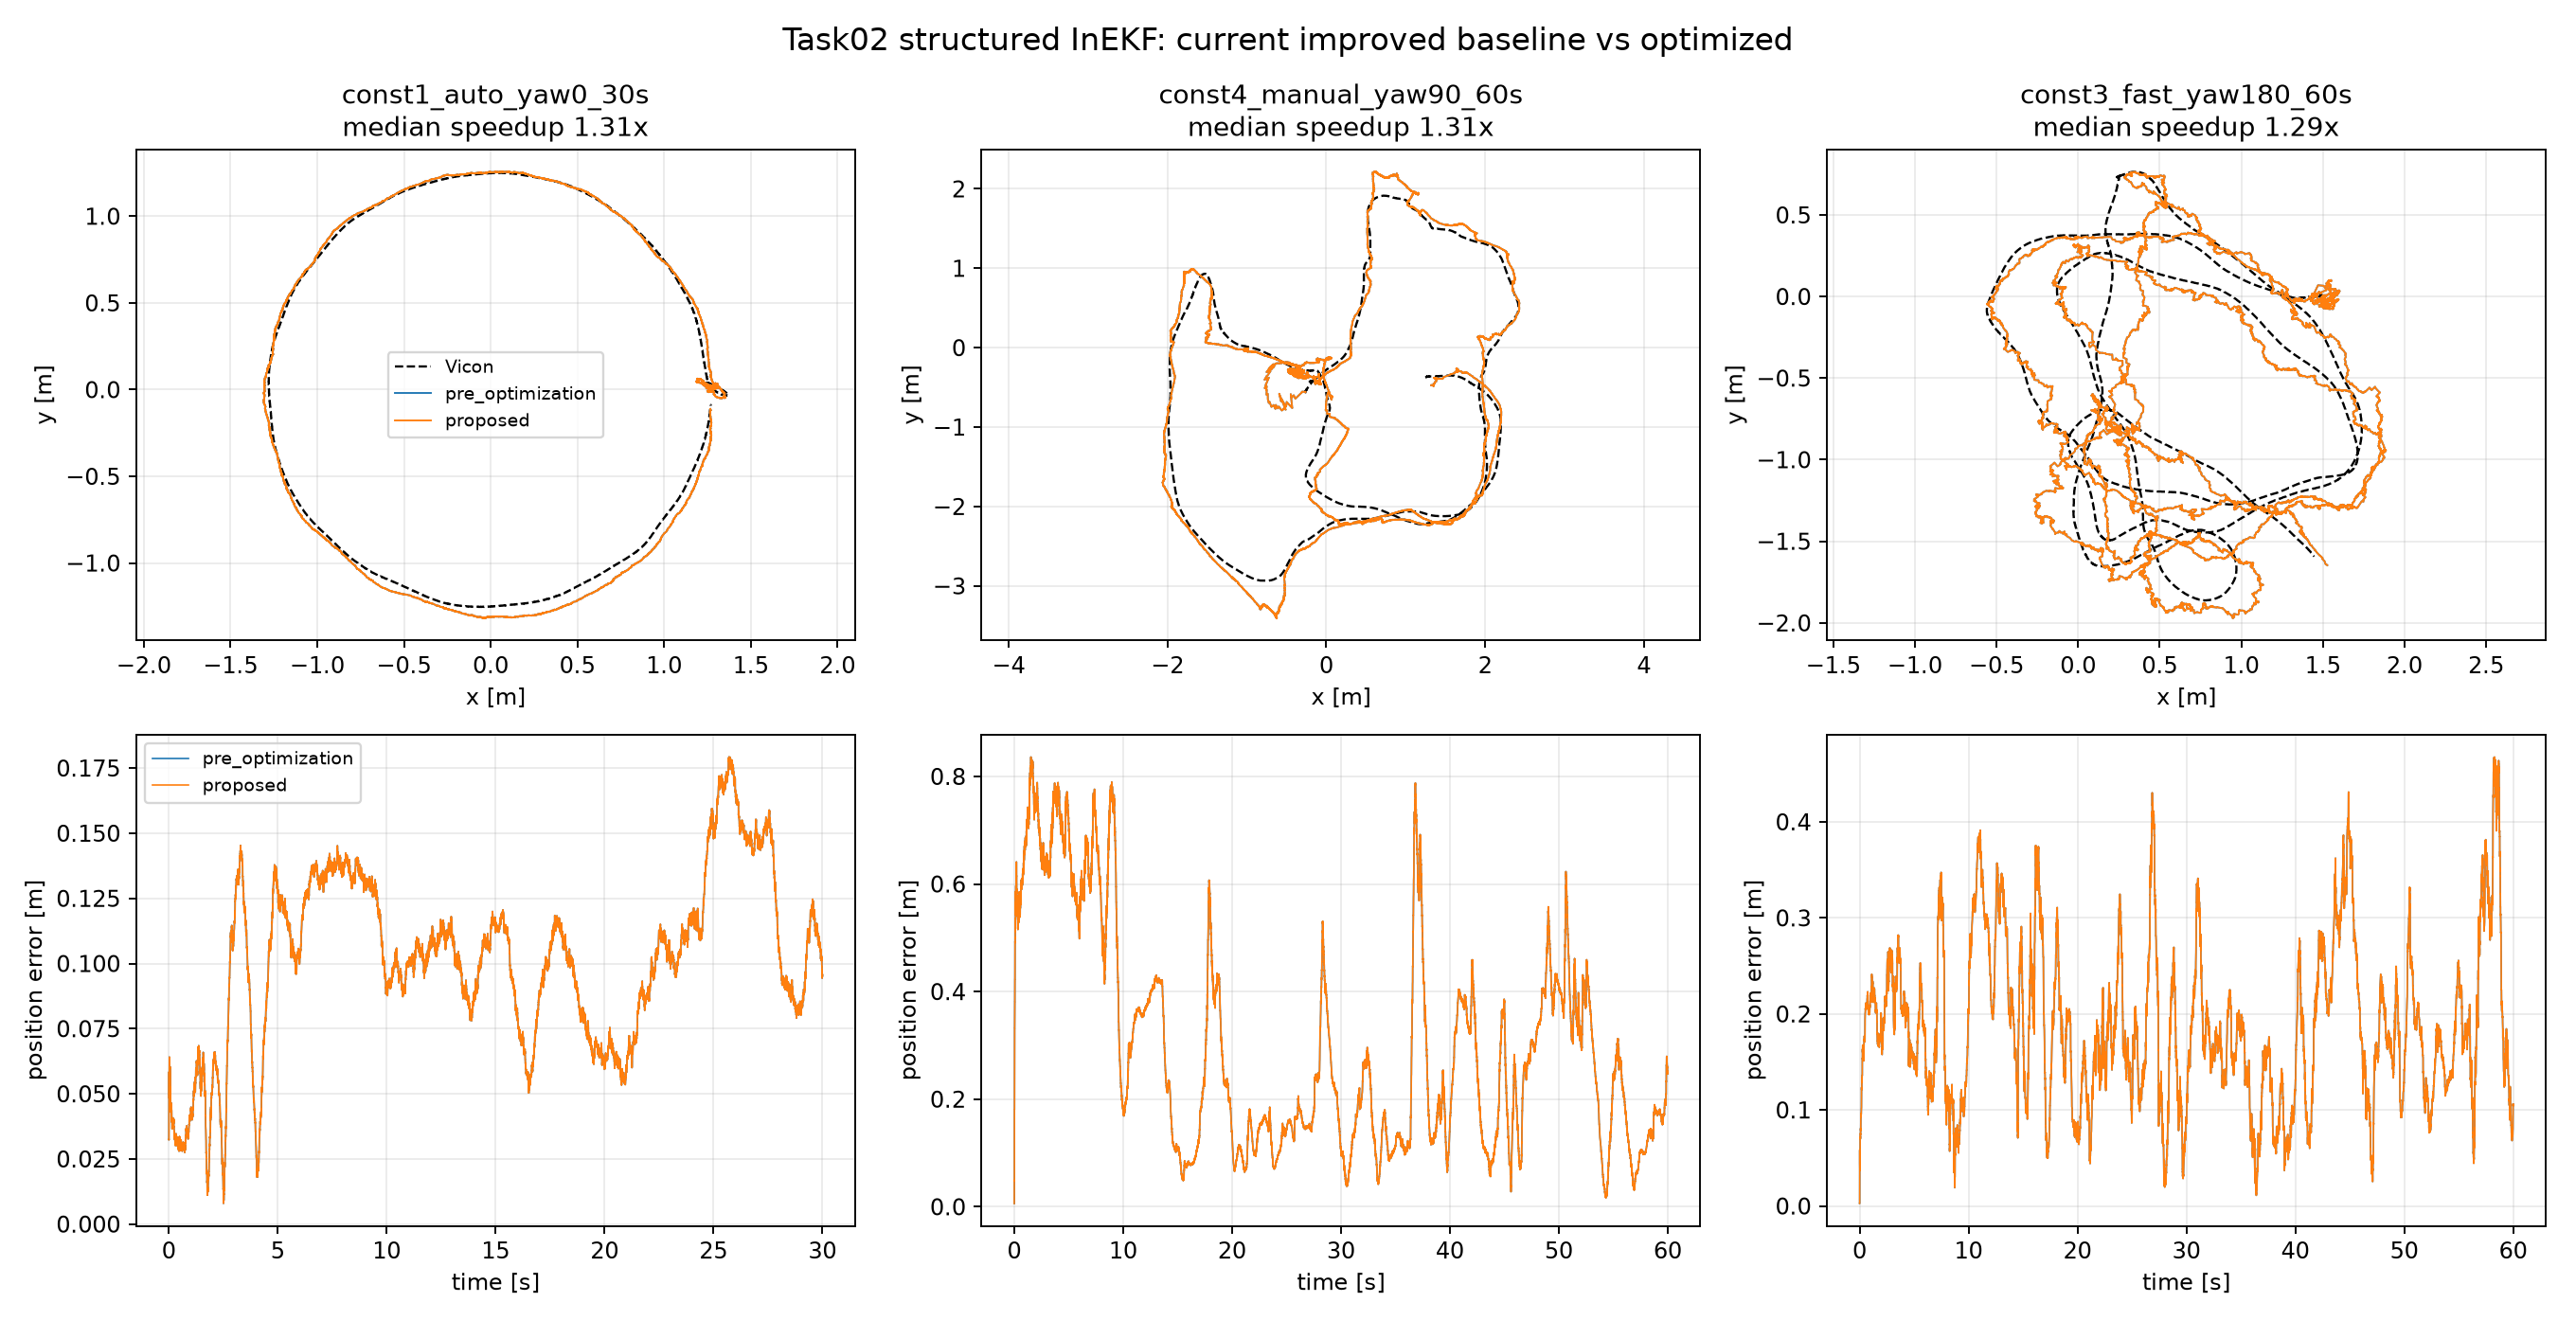
\includegraphics[width=\textwidth]{../imu-uwb-inekf/results/task02_optimization/comparison.png}
\caption{轨迹与位置误差。蓝色和橙色曲线几乎重合，未出现跳变或发散。}
\end{figure}

\section{结论}

本版没有以降维、降频或放宽门限换速度。受控配对回放得到约
1.29--1.31 倍端到端加速，同时保持大初始 yaw 收敛和 UWB 拒绝决策。
进一步显著降算力需要目标硬件上的固定尺寸分块核或多速率协方差传播，并应先补充
NEES/NIS 与采样率不变性验证。

\end{document}
